\chapter{Architecture} \label{architecture}

The aim of this project was to investigate the possibility of creating a hardware accelerator for a machine learning algorithm. We decided implement a module that could support the \textit{the LeNet-5} \cite{LeCun1998} (see Figure \ref{fig_cnn}). It was chosen for the reason that it is one of the easier CNN architectures to implement, and the module is only intended as a proof of concept. The input image is relatively small compared to the other architectures mentioned in Chapter \ref{chap_related_work}, which greatly reduces the amount of intermediate storage needed on chip. In addition the size of the kernels are the same in both convolution layers, making us able to reuse the convolution hardware accelerator for both layers, without adding configuration logic for different kernel sizes. 

Sadly, creating a module that provides the full functionality of a CNN requires more time than what was available for this project. But we were able to realize part of the network, the forward pass of the convolution and the subsampling/pooling layer, in VHDL code. For future references we will refer to our architecture as \textit{Imagezor}. This chapter will describe its design and the reasoning behind it. 


\section{Imagezor's Architecture}

Imagezor takes \textit{n} images as input, $ I_1, I_2, \dots, I_n $, a single kernel $ K $, and outputs a processed image $ O $. Using the input images and the kernel it performs the operations of the convolution and subsampling/pooling layer for a single kernel. Thus the output $ O $ is a subsampled/pooled feature map that has been produced by convolution the images $ I_1, I_2, \dots, I_n $ with the kernel $ K $. 

Imagezor can compute the convolution and subsample/pooling layer by doing the above computations for all the kernels in the respective layer. Thus one can exploit inter-parallelism by making several instances of the Imagezor architecture run in parallel. One can also exploit intra-parallelism, but then one need to connect the different Imagezor instances so they can add up the results from the convolutions without using the intermediate convolution buffer, as described in \cite{Chakradhar2010}.


Imagezors pipeline consists of five major components (Figure \ref{fig_imagezor_architecture}):

\begin{itemize}
	\item \textbf{The convoluter}. Performs the convolution operation on the input.
	\item \textbf{The intermediate convolution buffer}. Since the resulting feature map is the sum of the convolutions of all the input images (with the exception of the first layer), this buffer is needed to store the results from the previous convolution, so that it can be accumulated with the current convolution. In the first layer of the network there is only one input image (i.e. $ n = 1 $), thus no summation is needed.
	\item \textbf{Bias register}. Contains the bias value, and adds it to each convoluted pixel. 
	\item \textbf{Sigmoid}. Performs the non-linear sigmoid function  on the feature maps.
	\item \textbf{Subsample/max-pooler}. Performs the subsample/max-pool operation on the feature maps. 
\end{itemize}

\begin{figure}[h!]
	\centering
    	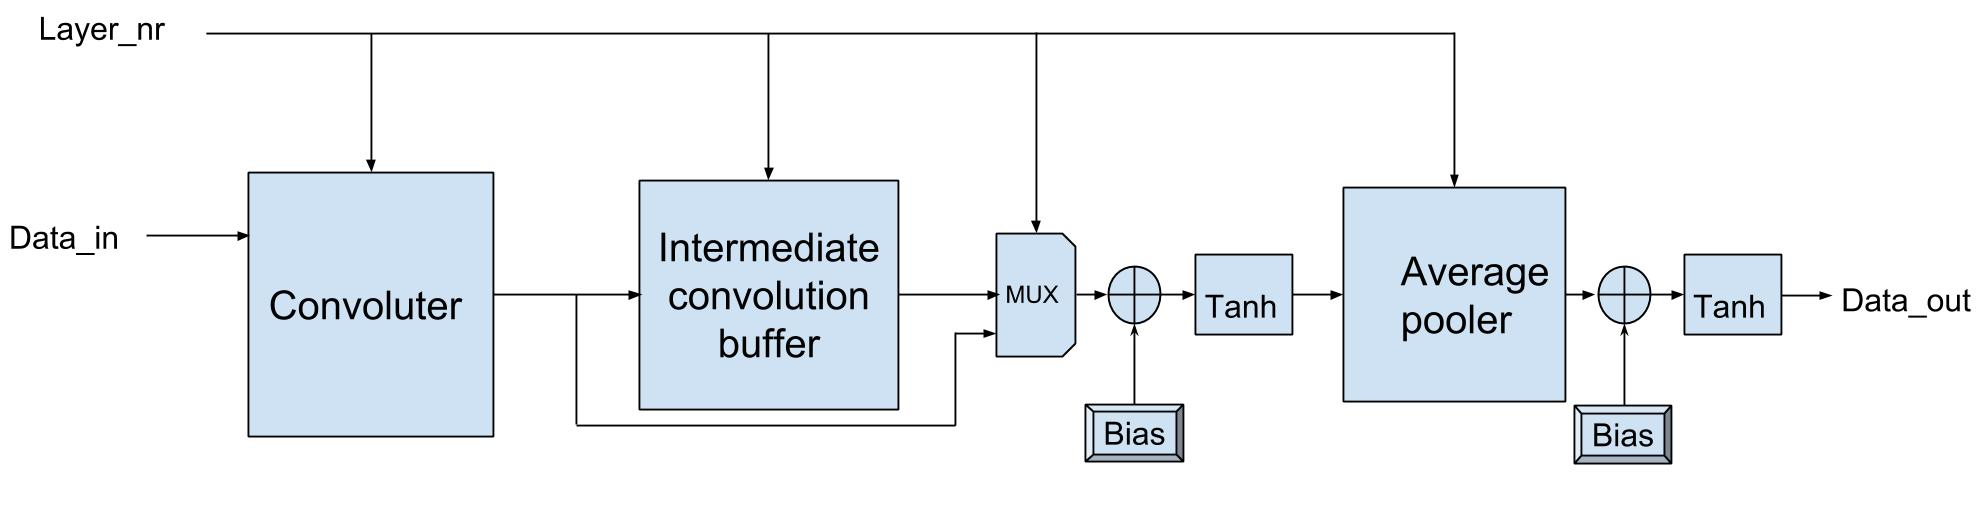
\includegraphics[width=1.0\textwidth]{Figures/Method/conv_layer_arch}
  	\caption{The architecture of Imagezor.}
  	\label{fig_imagezor_architecture}
\end{figure}

The \textit{layer\_nr} signal is used to define if it is the first or the second layer that is being computed. The input image in the first layer is bigger than in the second ($ 32 \times 32 $ vs $ 14 \times 14 $), which the convoluter and the max pooler need to compensate for (see Section \ref{sec_convoluter} and \ref{sec_max_pooler}). In addition in the second layer the intermediate convolution buffer needs to be activated so it accumulate and store all the convolutions needed to compute a single feature map. Thus the mux is needed to propagate the data directly from the convoluter in the first layer, and from the buffer in the second layer. 

Using this design one can compute a subsampled/pooled feature map with a single macro instruction. Thus it is the software's job to make the data available for the module in some kind of buffer, and then module will perform the actual computations.


In order to reduce resources spent and execution time, Imagezor uses Q8.8 fixed-point arithmetic, which is shown to give virtually the same network accuracy as floating-point arithmetic\cite{Napocensis2009} \cite{Holt1993} \cite{Chen2014}. 

In the sections below we will provide a more detailed description of the convoluter, the sigmoid unit and the max pooler. 


\subsection{The Convoluter} \label{sec_convoluter}

This module is inspired by \cite{Farabet2009}. The input is a $ n \times n $ image, and the output is a $ (n-k+1) \times (n-k+1) $ feature map, using a $ k \times k $ kernel. The kernel is stored in internal registers that must be rewritten for each different feature map that is to be computed. Every clock cycle the module takes in a pixel as input, and after a certain delay it will output a processed pixel almost every cycle. Each pixel is inputted once, left to right, one row at a time. 

It consists of 2D grid of multiply and accumulate (MAC) units which represents the convolution kernel. Thus the grid dimension is equal to the kernel dimension. In every MAC unit there is a register that contains the respective kernel weight. In every clock cycle the MAC units multiply the input pixel with its weight, and then accumulates the result from the previous cycle of the MAC unit to the left. 

At the end of each row of MACs there is $ n - k $ shift registers. The result of the last MAC in each row is stored in the first shift register, and the first MAC in each row takes the value of the last shift register of the previous row as accumulation input. The exception being the absolute first and last MAC unit. Every clock cycle the values in the shift registers are shifted to the right. 

\begin{figure}[h!]
  \centering
      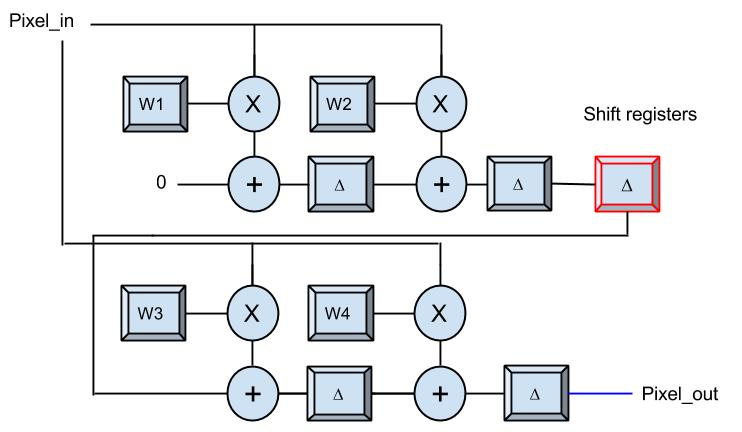
\includegraphics[width=0.7\textwidth]{Figures/Method/Convolver}
  \caption[The convoluter ]{The convoluter, when $ n = 3 $ and $ k = 2 $.}
\end{figure}
	
By providing this delay you only have to input each pixel once during the convolution. Generally every pixel is needed for $ k \times k $ convolution operations (the exception being the pixels close to the boarders of the image). Thus the shift registers are used to store the intermediate values of the convolutions until a pixel that is needed for the respective convolution operation is inputted. 

The delay these shift registers cause are the reason for the delay before valid output pixels are produced. Thus from when the convolution starts, the output will not be valid before $ k-1 $ rows of the image have been processed. And for every new image row, there will be a $ k-1 $ cycle delay before the output is valid. This is demonstrated by the fact that the input image is a $ n \times n $ matrix, while the output matrix is a $ (n-k+1) \times (n-k+1) $ matrix. 

Since the two layers in the network have different image sizes, but uses the same kernel size, we can reuse the module for both of them. This is done by having the control signal \textit{layer\_nr} decide how many of the shift registers that are to be used during convolution. In the first layer all of the shift registers are used, but in the second only a subset is used. I.e. $ n-k+1 $ of shift registers are used in each row, where $ n $ is either 32 or 14. 

The loading of the weights takes $ k \times k $ clock cycles, and the processing of the image takes $ n \times n $ clock cycles. Thus the total number of cycles it takes to perform a full convolution of an image is $ n \times n + k \times k $. But based upon the papers refered to in Section \ref{sec_related_work} it seems that \textit{n} tends to be larger than \textit{k}. E.g. for the first layer in the LeNet-5 \cite{LeCun1998}, $ n = 32 $ and $ k = 5 $, the loading  of the weights take 25 clock cycles and the image processing 1024 cycles. This means that the execution time of the convoluter is primairly bounded by the size of the image. But the size of the kernel decides the hardware resource cost of the module, since it requires $ k \times k $ DSP slices on the FPGA. Thus the 32 DSPs on the Spartan 6 is enough in order to implement the LeNet-5. 

\begin{figure}[h!]
  \centering
      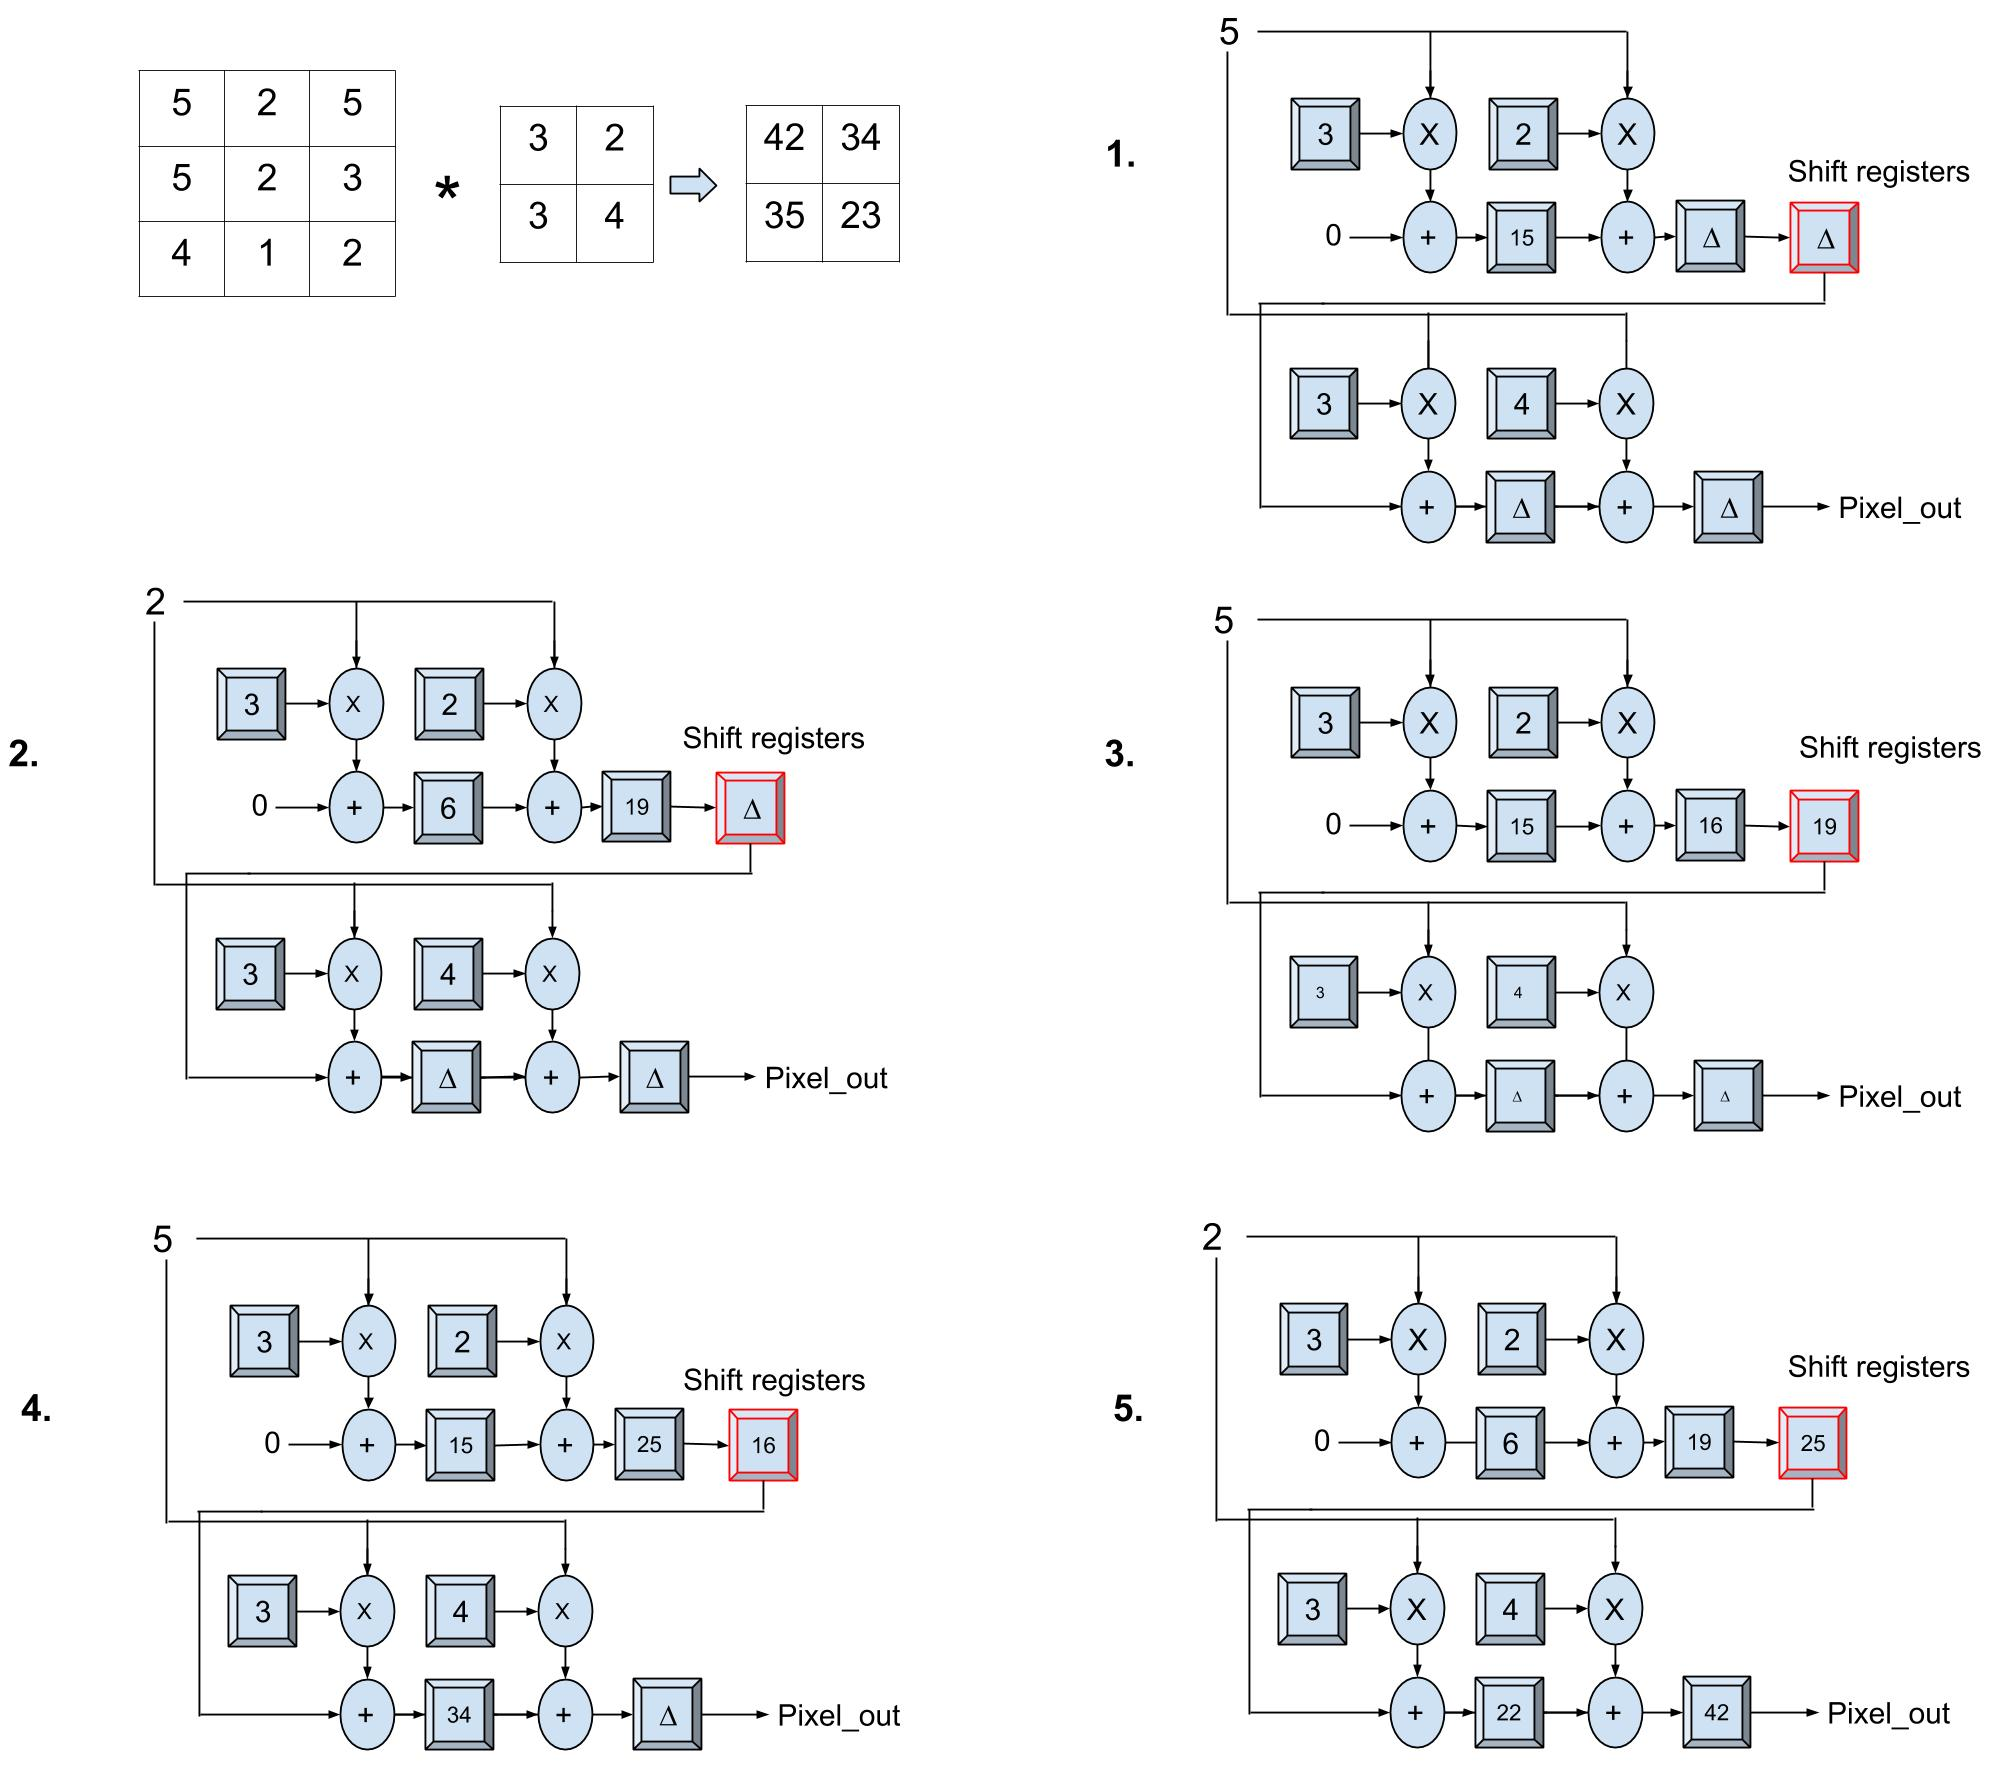
\includegraphics[width=1.1\textwidth]{Figures/Method/Conv_example}
  \caption[Convolution example]{Example showing the five first clock cycle of an convolution. The weights of the kernel is already loaded into the MAC units, and every cycle a new pixel from the image in inputted. In the last example you can see that 42 is provided as the first output.}
\end{figure}

\subsection{The Sigmoid} 

This module is based upon \cite{Napocensis2009} using PLAN approximation. It takes input a single value \textit{x} and outputs a linear approximation of the sigmoid function. Using a lookup table (Table \ref{tab_sigmoid}) the module decides which linear approximation to use.


\begin{table}
	\centering
    \begin{tabular}{| >{\centering\arraybackslash}m{2in} | >{\centering\arraybackslash}m{1.2in} |} 
    \hline
    PLAN(X) & Conditions \\ \hline
    1 & $ |x| \geq 5 $ \\ \hline
    $ 0.03125 \times |X| + 0.84375 $ & $ 2.375 \leq |x| \le 5 $\\ \hline
    $ 0.0125 \times |X| + 0.625 $ & $ 1 \leq |x| \le 2.375 $\\ \hline
   	$ 0.25 \times |X| + 0.5 $ & $ 0 \leq |x| \le 1 $\\ \hline
    \end{tabular}
    \caption{The PLAN approximation of the sigmoid function.}
   	\label{tab_sigmoid}
    
\end{table}

\vspace*{1\baselineskip}
\subsection{The Max Pooler} \label{sec_max_pooler}

The max pooler performs the subsample/max-pooling operation described in Section \ref{sec_cnn_def}. The input is a $ (n-k+1) \times (n-k+1) $ feature map, and the output is a $ (n-k+1)/p \times (n-k+1)/p $ subsampled/max-pooled feature map, where \textit{p} is the dimension of subsample neighborhood. As with the convoluter, one pixel is streamed in every cycle, and streamed out whenever a valid pixel is ready. Designed this way the max pooler can process in parallel with the convoluter, by directly streaming the output of the convoluter into the max pooler module. In other words, the operations of convolution layer and subsampling/pooling layer is pipelined.

\begin{figure}[h!]
  \centering
      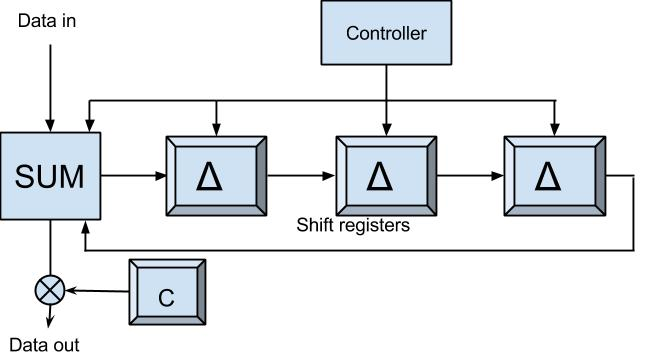
\includegraphics[width=0.5\textwidth]{Figures/Method/submax}
  \caption{The max pooler.}
\end{figure}

The module compares the input with the current max value, and updates the max value accordingly. It contains a set of \textit{(n-k+1)/p} shift registers. Since the image is divided into $ p \times p $ non-overlapping neighborhoods, the module needs to store the current maximum value of previous neighborhood when a pixel from a new neighborhood is inputted. To do this the module contains two counters, \textit{row\_num} and \textit{column\_num}. When a new pixel is inputted the \textit{column\_num} counter is incremented, and when a new row is encountered the \textit{row\_num} counter is incremented. Every time $ column\_num~mod~p = 0 $ the shift registers are shifted one to the right, and every time $ column\_num~mod~p = 0 $ and $ row\_num~mod~p = 0 $ a valid output is produced. 



The execution speed of the max pooler module is bounded by the size of the feature map, $ (n-k+1) \times (n-k+1) $ clock cycles, finishing one cycle after the last pixel has been inputted. 
Thus by streaming the output of the convoluter to the max pooler, both will finish only a few cycles apart, effectively running both jobs in parallel. The resource usage of the module is bounded by the size of the subsampling dimension, since it requires a number of shift registers equal to the size of the dimension. But essentially its resource usage is quite low.  
